%!TEX root = ../dissertation.tex
\chapter{Amortization: Memory as a computational resource}
\label{chap:amort}

In this chapter, I introduce the concept of \textit{amortization}. This refers to spreading costs over a period of time. In our case, these are computational costs that can be amortized by re-using parts of previously computed solutions. Therefore, simply by remembering past solutions to problems, and flexibly re-using them in the face of new problems, we can use memory as a computational resource to ease the burden of real-time computation to solve these new problems. 

In this chapter, I will first discuss the computational problem that amortization addresses. I then discuss how it links to ecological rationality, as well as outline how it might be implemented. Finally, I discuss amortization in models of human cognition.

\section{Two kinds of knowledge}

There are two distinct aspects to making an inference. The first is the have the relevant information from the external world that will best inform that inference. This usually means having a good model for how that aspect of the world works. Once we have this information, it is in theory possible to make optimal inferences. But such these optimal inferences remain to be computed from this information. The second aspect therefore is to actually perform the computations that result in an inference, and compiling abstract understanding of the world in the form of a model, to an actual response. We refer to the first kind of information as `potential knowledge', since all optimal inferences are in theory possible to compute, once we have an accurate model of how the world works. We refer to information obtained by actually computing inferences in such a model as `realized knowledge'. 

We give an example for intuition. Once we learn the rules of mathematics, the proofs of all the theorems in the world are included in potential knowledge. However, only a small subset of these proofs can and will actually be computed by anyone who knows the rules of mathematics. This subset is realized knowledge. Arriving at each of these proofs requires some work. Even if we already know enough about a domain works suggest that all potential knowledge is within reach, going from that to realized knowledge can require prohibitive amounts of computation. These computations cost resources. It is these costs that we wish to amortize. Since we are concerned primarily with the computations involved in going from potential to realized knowledge, we assume that potential knowledge has already been acquired and what remains is to compute realized knowledge, and discuss how the costs of this procedure might be amortized.

\section{Amortization and ecological rationality}

As mentioned earlier, we assume for now that we already know how the world works, and all potential knowledge is within reach. When faced with a new query, the challenge is in performing the computations that go from this potential knowledge to an (approximately) optimal response to this query. This might require extensive computational resources. If these is structure in the space of queries observed -- such that similar queries appear often -- then it is wasteful to recompute response to each query independently every time it is encountered. Instead, one could re-use parts of previously computed responses to similar queries. This amounts to amortizing the costs of computing a response to a query over many previously encountered similar queries, and using memory as a means for easing the burden of computation.

Amortizing the costs of computation is `rational' only if there exists structure in the environment that such that we expect some similarity in queries encountered. In different environments, with different distributions of queries, different levels of amortization can be optimal. For example, if a query is rarely experienced, there may not exist adequate previous experience to re-use. Further, the cost of storing and recovering previous solutions might not be worth the computational savings incurred from amortization -- especially if the possibility of it being encountered again is rare. However, when we have a large amount of experience in an environment, and there does exist some additional structure in the space of queries, it becomes more rational to amortize computations. I argue that the re-use of computations in such structured environments can lead to ecological rational behavior -- i.e. behavior that adapts to and exploits structural regularities in an environment. 

This mechanism for the arisal of ecological rationality addresses some of the concerns raised in Chapter \ref{chap:psych} about how ecologically rational behavior might come about. To briefly re-iterate the concern, while heuristic behavior in humans has been characterized an ecologically rational\cite{gigerenzer2008heuristics}, they largely remain `as-if' models -- that show that the heuristics implemented in human inference are `as-if' humans are implementing ecological rational shortcuts. But it remains to be understood how these heuristics arise, and further, how one chooses the right heuristic for the right environment -- with the computations required to make this choice often being comparably expensive to computing the optimal response from scratch\cite{lieder2017strategy}. The mechanism of simply reusing the procedures that worked well for previously encountered queries in an environment, by amortizing the computations that go into computing these responses, allows for a feasible way to implement ecological rational behavior. 

The intuition for this is as follows. We likely do not encounter random queries in an environment, rather, we expect there is significant structure in the queries we regularly compute responses to in an environment. For example, our generative model of how physics works could allow us make reasonable predictions for abstract questions like where we expect a ball thrown at a random angle to fall. However, most of our personal experience making such a prediction might be not from making these abstract judgments. A more common use case for making such predictions might be to gauge the motion of a ball thrown at us, with the intention of catching it. Excellent performance on this task can be achieved simply by applying a \textit{gaze heuristic}\cite{gigerenzer2009homo}: by fixating one's gaze to the ball and adjusting running speed so that the angle of the gaze remains constant while approaching the object. This heuristic is much simpler to implement than making optimal inferences in a complex generative model of projectile motion -- however, this only works for this specific subset of all the ways in which balls could be thrown and does not generalize to all projectile motion problems.

Previously encountered problems in this domain are biased towards these more common queries. Therefore amortization of past computations, performed to respond to these biased set of queries, will also reflect this structure. This leads to a bias that makes inferences that are likely to occur in an environment easier, but does not fully represent possible complexities in the full space of all possible queries -- i.e. it leads to an ecologically rational heuristic. Application of such a heuristic could therefore lead to errors on uncommon queries.

In the following sections, as well as in later chapters, I will expand upon this connection. I will also discuss how taking closer account of the environment in determining the ecologically rational inference procedures learned can better inform not only our understanding of human cognition, but also of artificial intelligence, and can generalize this understanding across a wide array of domains.


% We discuss how different amortization strategies can arise depending on the structure in the environment and limitations on computational resources, and outline empirical evidence for these behaviours in natural intelligence.

\section{Forms of amortization}

Amortization can take many forms. The most general approach is to think of the computations amortized over previous experience as a sort of `response-prior' for new queries. Note that this is distinct from the prior over hypotheses in the domain we are carrying out inference. That is included in `potential knowledge' and we assume it has already been learned. The response-prior is information gained from previous computations -- when going from potential to realized knowledge in past queries. Crucially, we already possess the knowledge to make an optimal inference from scratch, the response-prior simply provides heuristic, unstructured information that makes arriving at a good inference -- i.e. going from potential to realized knowledge -- computationally cheaper. The response-prior can therefore take many forms. For example, it could inform the type of optimal response (e.g. it is usually one or two words long), the rough location of the optimal response (e.g. it's usually between 10 and 40), heuristic strategies for arriving at good responses (e.g. the best option is often the 2nd most expensive one), or similarity functions to previous episodes (e.g. do exactly what I did last time I was playing a similar game, because that worked). 

I briefly discuss the key principles behind how amortization is possible in the various algorithms for approximate inference discussed in Chapter \ref{chap:approx}. These will be discussed in greater detail in Chapters \ref{MCMC_amort} and \ref{chap:LTI}.

\paragraph{Amortization in a sampling framework} 

In a Monte Carlo framework, what can be re-used query to query are the samples themselves -- or certain summary statistics of the samples. Consider an example where we have samples from the space of hypotheses $h \in \mathcal{H}$, sampled from the posterior distribution $P(h | d)$, giving an approximate distribution $\hat{P}(h | d)$ . Supposed we generated these samples in response to a query that demanded the posterior probability of a specific hypothesis $h_1$. The approximate responses in this case would be $\hat{P}(h_1 |d)$. Now, if we are asked another query about the posterior probability of a different hypothesis $h_2$. Note that if we store these samples and re-use them for this new query, we don't have to do any new computations -- the sample-based approximate distribution $\hat{P}(h | d)$ can be used to respond to this new query without any additional samples drawn. However, storing all the samples might be very intensive on memory. One possibility is that people instead store certain statistics of the samples instead. While this reduces how much flexibility we have in the kinds of the re-use we might want, it reduces load on memory. We propose more specific algorithms for amortization in a sample-based approximations, as well as test them in humans in Chapter \ref{chap:MCMC_amort}.

A disadvantage of purely sample-based re-use is that it is less flexible when two queries are not querying the same posterior distribution. The framework described so far provides no way to re-use samples from $P(h | d)$ in $P(h | d')$. We will see in Chapter \ref{chap:MCMC_amort} however, that humans re-use inferences flexibly across different posterior distributions as well. I model this with re-use in a variational framework in Chapter \ref{chap:LTI}. I outline below briefly what this kind of re-use could look like below.

\paragraph{Amortization in a variational framework} 

In a variational framework, the approximate posterior $\hat{P}(h | d)$ is a member of some parametrized family that we choose as the variational family. These parameters therefore can be re-used from query to query. A key advantage of representing the approximate posterior as a finite set of variational parameters, rather than a variable number of random samples, is that it makes it easier to flexibly re-use inferences. I outline below how this might be possible.

In Figure \ref{fig:var_schematic}, we introduced a schematic for variational approximation. To better understand flexible re-use in this framework, we consider a variant of this schematic in Figure \ref{fig:var_schematic_amort}. The key observation here is that a variational approximation determines a mapping from inputs (priors, likelihoods and data) to the output (a posterior approximation). One path to go from the input to the output is to explicitly solve the variational problem. Over extensive experience in a domain, we will have solved this variational problem for a variety of inputs. Therefore, we have built up a large number of such input-output pairs. We are therefore in a position to see if there are any patterns in this mapping from input to output, that we can use to best inform future computations. This can be done by simply learning a regression function, from previous input-output pairs, that maps a query (data, prior, likelihood) to an output. \footnote{The inductive biases we use in the regression function that we learn will influence the outputs predicted for new inputs. See Chapter \ref{chap:LTI} for a more detailed discussion of this.} When faced with a brand new query -- that is different from other faced before, but might have certain similarities, this mapping allows us to immediately have a good guess for the approximate posterior. This can be further optimized using the standard optimization procedure used for variational inference, but will require fewer steps of optimization, and fewer computational resources, since our initial guess is well-informed. In this way, we can use information gathered from previously computed input-output pairs to amortize the cost of finding variational approximations for new inputs. In Chapter \ref{chap:LTI}, we show that many errors and biases observed in human probabilistic judgment are explained by this mechanism.

\begin{figure}[t!]
\centering
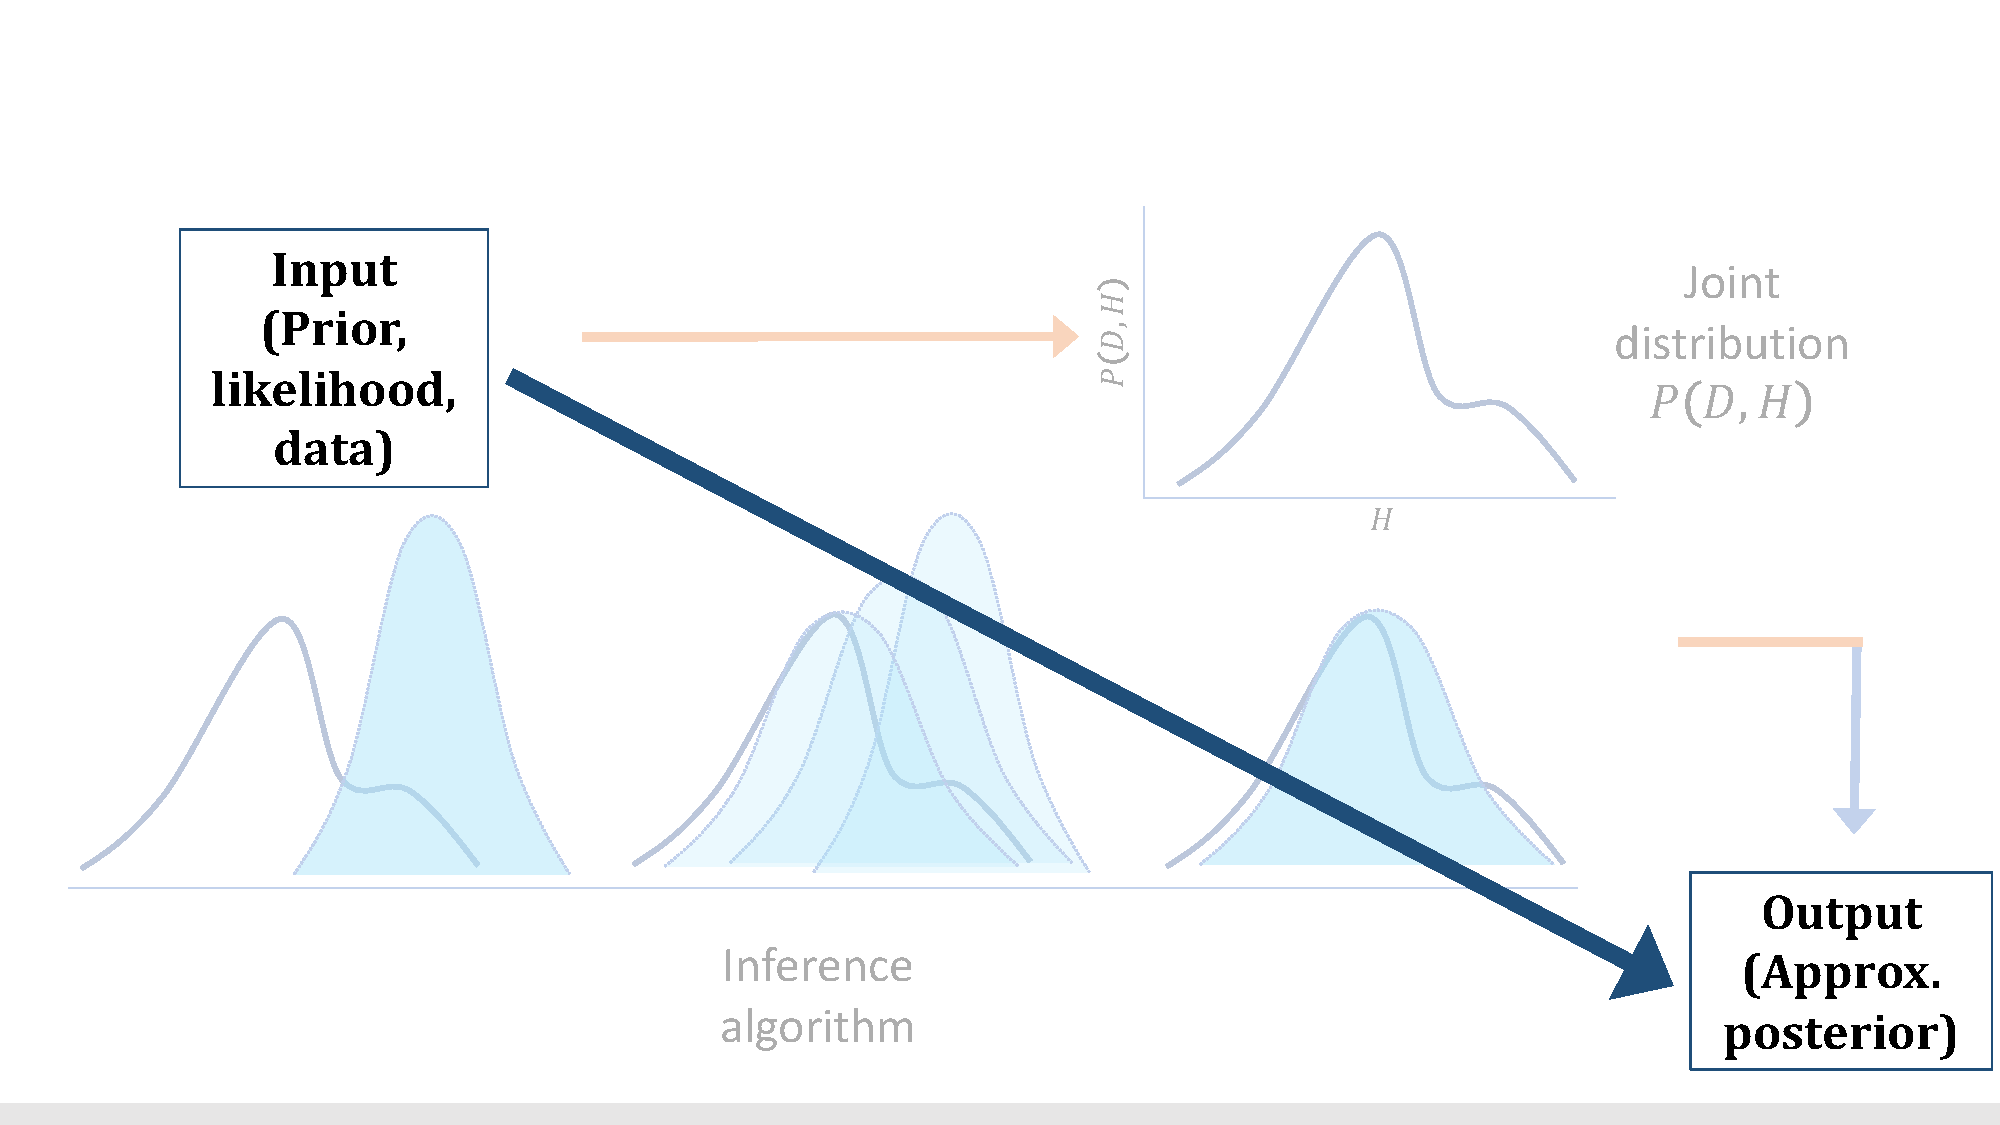
\includegraphics[width = \textwidth]{figures/var_schematic_amort.pdf}
\caption{\textbf{Schematic for Amortized Variational approximation}. }
\label{fig:var_schematic_amort}
\end{figure}

Variational approximations still have the disadvantage that they have no asymptotic guarantees, while sampling methods do. A promising way forward is to combine the complementary advantages. Most Monte Carlo approximations rely on having a good `proposal distribution' -- that closely approximates the true posterior -- in order to converge quickly and provide good approximate posterior probabilities under realistic limitations on the number of samples. We expect humans to be in this low sample regime when using Monte Carlo methods, due to the limitations imposed by their cognitive limitations. Variational approximations could provide this proposal distribution. This way, we can retain the flexible re-use permitted by variational inference, as well as the asymptotic guarantees of sampling. This possibility is discussed in greater detail in Chapter \ref{chap:LTI}.

\section{Amortization in cognitive science}

It is an uncontroversial observation in cognitive science that experience in a certain domain and greater familiarity with it leads to easier, faster, almost automatic inferences. Amortization offers an explanation for this phenomena. As phrased by \citet{logan1988toward}:
\begin{quote}
``Automaticity is memory retrieval: Performance is automatic when it is based on single step direct-access retrieval of past solutions from memory. The theory assumes that novices begin with a general algorithm that is sufficient to perform the task. As they gain experience, they learn specific solutions to specific problems, which they retrieve when they encounter the same problems again.''
\end{quote}
Amortization formalizes this notion of flexible re-use of past computations, despite already having a `general algorithm sufficient to perform the task', which in our case is performing inference on the already known model of the world. 

This results in a dependence on the history of queries observed, leading to another key prediction of amortizing inference. If there is additional structure in this historical query set, we expect the development of ecologically rational shortcuts that reflect this structure. These shortcuts might give close to optimal responses on commonly observed queries, but would give poor performance on uncommon ones. This provides a potential explanation for some kinds of biased inference in humans. We will also see how this can inform inference procedures learned in artificial systems. Note that if computations were being carried out from scratch -- computing realized knowledge from potential knowledge each time -- there would be no difference in behavior between common and uncommon queries.

Here, I discuss how amortization has been an implicit part of many approaches to  in models of human cognition, focusing in particular on two domains: Inference and planning. Planning can be seen as a specific case of inference\citep{botvinick2012planning}, but these have historically been studied as separate problems, with various approaches to each developing independently. So we first address amortization in these two separately and then discuss how the methods developed in each can better relate and inform one another, when seen through the common lens of amortization.


\subsection{Amortization in Inference}

%In the problem of exact Bayesian inference discussed in Chapter \ref{chap:approx}, the goal is to make a judgment about posterior probabilities $P(h | d)$.  From this potential knowledge, we can in theory then compute posterior probabilities (i.e. realized knowledge), but this step comes with the computational costs of performing exact or approximate posterior inference.

In many real-world situations, people have to combine information from many sources, in order to make judgments about probabilistic outcomes. As discussed in Chapter \ref{chap:psych}, Bayesian inference provides a normative computational account of what should be done. The first step in Bayesian inference is acquiring the requisite potential knowledge  -- i.e. to collect information from the world in order to inform a joint distribution $P(h,d)$. This includes learning a prior distribution $P(h)$ as well as a likelihood function $P(d | h)$. We will assume that this step is already complete. The second step, that we focused on in Chapter \ref{chap:approx} is of going from the possible to realized knowledge. That is, of computing normalized posterior probabilities  $P(h |d)$. Given data $d$, Bayes' rule stipulates how a rational agent should update its prior probabilistic beliefs $P(h)$ about hypothesis $h$:
\begin{align}
    P(h|d) = \frac{P(d|h)P(h)}{\sum_{h'} P(d|h') P(h')},
\end{align}
where $P(h|d)$ is the agent's posterior distribution, expressing its updated beliefs. In case of many underlying hypotheses (as is often the case), this denominator is difficult and often intractable to calculate. Therefore, despite having the requisite `possible ' knowledge in the form of the generative model $P(h,d)$, the `realized' knowledge of the posterior probabilities are non-trivial and remain a computational challenge.

Amortization suggests that this computation be spread out over previously encountered queries, resulting in response priors that bias inference. Evidence that this might be happening in human cognition would be if experts are more likely to use heuristic strategies than novices -- given the same domain information. The use of heuristic-based strategies has been observed in experts in various domains such as legal decisions \citep{dhami2001bailing}, and medicine \citep{reyna2006physician}, where the most general, normative decision strategy involves several variables and is often too complex for easy full consideration. \cite{garcia2009take} find, in a domain of criminality and law enforcement, that expert behavior is better described by heuristic strategies, while laypeople are better described by a full regression to the relevant variables. These provide preliminary evidence that these heuristic strategies are in fact learned, from experience. Amortization provides a mechanism for this.

In thinking of a heuristic as a learned function from query to response, the role of memory becomes more obvious. Previous experience stored in memory, provides a set of input queries and output responses -- where the response was either computed using a noisy general purpose, normative strategy, or externally provided say by a teacher. These pairs can be used to fit a function, i.e. find a heuristic, that is separate from the normative decision strategy. This also alleviates the startegy selection problem because it isn't that people come in with an arsenal of heuristics and then select one, but rather learn a heuristic via historical experience in that domain. Previous work \citep{gluck1988conditioning, dasgupta2019theory, shanks1991connectionist} has demonstrated that different approximate solutions to general-purpose probabilistic inference can arise from such a mapping, and that these vary depending on the distribution of queries. 

%Also integrates with episodic re-use of specific examples (connection to \cite{dasgupta2018remembrance}), by informing when to re-use (analogous to episodic RL, learning a similarity function).

\subsection{Amortization in Planning}

While the main focus of this paper is on inference and not planning, amortization has implicitly played a very crucial role in our understanding of how planning might be implemented. In this section, we briefly review the literature on how amortization fits into the existing framework for approximate planning. We then discuss how these might inform our primary discussion on amortization in inference.

The goal of planning is to leverage information one has about the world in order to achieve a specific goal. This problem has been commonly studied in a Markov Decision Process paradigm, in the context of Reinforcement Learning (RL). The framework here is that an agent has a fixed set of actions ($a \in A$) it can perform on the world, in order to receive reward ($r$). This reward depends on both the state of the world the agent is in ($s \in S$) as well as the action taken, as defined by a reward function $r = R(s, a)$. The goal is to maximize this earned reward, over some fixed or discounted time horizon. The effect of an action will depend on the state of the world the agent is in, and can cause a transition from one state $s$ to another state $s'$ as defined by a transition model $P(s' | s, a)$. A common assumption, that makes the problem more tractable, is that the transitions and reward structure are Markov -- i.e. that when taking action $a$ in state $s$, which state we transition to ($P(s' | s, a)$) as well as the reward earned ($R(s,a)$) depend only on the current state and current action and is independent of the history of any previous states or actions.

In a planning problem, the transition probabilities and reward functions are known -- this consists of all the potential knowledge about this domain. The challenge in converting this to realized knowledge is to construct a \textit{policy} $\pi: S \rightarrow A$ that determines what action to take at each state, in order to maximize the reward earned. The number of possible trajectories through the MDP is exponentially large, and evaluating every possible policy -- despite already having all the potential knowledge in the domain -- is computationally very challenging and often entirely intractable. Amortization of previous computations, to better inform a policy, is a common approach to easing the burden of planning.

% \footnote{In contrast with our discussion on possible vs realized knowledge in an inference setting, the traditional RL setting does not assume all possible knowledge is, the transition probabilities and reward functions are not assumed to be known, and also needs to be learned from experience. Most established approaches in this domain therefore do not keep these two kinds of learning distinct -- we will primarily be discussing the planning problem, but most discussions will relate back to the broader RL problem as well.

% In the most general form of the problem, the agent does not know which state it is in and must additionally infer the state it is in from observations O. If an observation does not uniquely identify the underlying state, then the Markov assumption no longer holds. The goal is to learn a policy i.e. a mapping from observations to action, that maximizes reward.

Since approximate planning has largely been studied under the broader banner of RL, we first note an important distinction between our discussion of amortized Bayesian inference and the standard RL paradigm. We previously assumed that all possible knowledge of the world has already been acquired, and the only challenge left is it converting this to realized knowledge. While this is still true of a pure planning problem, the standard RL paradigm simultaneously learns both. The two traditional approaches to the RL problem are: a) learn a world model i.e. learn the states, as well as the reward and transition structures. This amounts to acquiring all potential knowledge. Using these, we can predict the outcome of possible actions in this model and choose actions that lead to reward. This approach is often termed model-based RL. Finding the right response at run-time is a planning problem, and is expensive -- although it guarantees optimal responses. The second approach is b) to directly learn which actions lead to reward through experience. This is done by trial and error and is often termed model-free RL. In this approach, flexible possible knowledge is not even stored, and is stored directly as realized knowledge. A general form of model-free RL is to learn a `value function', that simply takes in a state and action, and return the expected reward over the relevant time horizon (also called the `value') of taking that action from that state. Therefore finding the right response at run-time is very cheap -- it simply involves finding the action that maximizes value as determined by the value function.

To better draw parallels to our discussion of amortization in inference, we consider a hybrid between model-based and model-free systems, namely the DYNA architecture, or the wake-sleep architecture. Here, the model is learned and stored i.e. all potential knowledge is explicitly acquired. However, every time a computation in this model is carried out leading to an actionable policy (i.e. realized knowledge), this computation is used to update a value function as well. Now, if another similar computation is demanded, it does not have to computed from scratch; the value function learned from previous experience can inform this computation. This can take the form of a `response-prior' that informs which state-action pairs seem the most promising, and thereby reduce the search space of exact planning. This amortizes the costs of exact planning. 

While evidence of both model-based as well as model-free behavior has been observed and extensively studied in human cognition, amortization via a DYNA-like architecture provides promise of a unification of the two via amortization. This consistent with 

Other approaches to RL have also implicitly invoked amortization of planning. The successor representation is an ecological rational adaptation to worlds in which the transition function $P(s' | s, a)$ does not often change, but the reward function $R(s, a)$ does. This implicitly amortizes computations by re-using past experience of transition probabilities. Episodic approaches to RL -- where the goal is to simply learn similarity functions to previous experience to facilitate adaptive re-use -- can also be seen as amortization. \footnote{A crucial caveat is that since the line between acquiring potential knowledge and computing realized knowledge is blurred in RL, it is more difficult to explicitly separate out the roles of learning about the environment and learning how to do fast computations with that knowledge in these examples.}

%Empirical evidence of such offline updating has been suggested and studied in the context of reinforcement learning via the DYNA architecture \citep{sutton1990integrated, gershman2014retrospective}, moral judgements via empathy-based appraisal \citep{ugazio2014empathy, van2016imaginative}, modal cognition via the evaluation of conditionals and counterfactuals \citep{ichikawa2012rational, phillips2018psychological, williamson2007philosophical, roese1997counterfactual}, and consolidation via replay (during sleep?, unsure if hippocampal reply can be characterized as `from a model' to a compiled response).


%The first is more flexible, since it allows one to predict the effects of actions in situations never previously encountered directly, and is quickly able to adapt its policy to changing reward structures. The second is less flexble since (in its most basic form), requires each observation-action pair to have been experienced in order to know its value. Further, if the reward structure changes, then all of these observation-action pairs need to be revisited in order to revise the new values of each of these. On the flip-side, the model-based strategy is very computationally expensive at run-time -- it requires the simulation of several steps into the future, and a combinatorially high number of possible trajectories to evaluate the value of an action. Whereas the model-free strategy uses previous experience in the domain to inform future the value of actions, and saves significant computational energy at run-time.

%The model-based representation is "possible knowledge" that is, it contains within it all the required information to maximize reward in the environment. However, compiling it into an actionable policy, is computationally expensive. The model-free representation however contains compiled knowledge that directly informs actionable policy, at the cost of throwing away the flexibility of abstraction. One way to integrate these advantages is to use a learned world model to perform planning in advance, and compile the results into rapidly recoverable query-response rules which can be easily used for real-time inference. This architecture is often referred to as DYNA, as was discussed briefly in the previous section. In this section, rather than overlaying these two approaches as with DYNA, we explore instead the continuum between these two diametrically opposite approaches. We investigate how various approaches to approximate planning can be seen as different points on an amortization spectrum. Here, the distinction between the two kinds of knowledge -- possible and compiled / realized -- is less clear since both have to be acquired. Instead we focus on how different frameworks trade-off abstraction (i.e. a flexible representation that encompasses all `possible' knowledge) and computational resources (i.e. a compiled response that represents `realized' knowledge and directly informs strategies). We outline how different points on this spectrum might be optimal for different environments, depending on the complexity of the world and the variability in the query distribution.

%Model-free value functions, pruning. Episodic RL. Temporal abstraction, options. Successor representation -- since much of the important structure in the environment is baked into the representation, simple computations with this representation can give good responses. 

\subsection{A fruitful exchange}

There are two crucial ways in which the study of amortized planning can better inform our study of amortization in inference.

First, the strategy selection problem -- a central issue the study of domain-specific, ecologically rational heuristics as a solution to bounded optimality -- has often been framed as meta-cognitive reinforcement learning problem. \cite{erev2005adaptation, rieskamp2006ssl, lieder2017strategy}. Here, an agent decides not only the actions it wants to take in the outside world, but also decides how much information to gather, how much time to spend, as well as how much cognitive energy to invest, in improving an inference. This can be formalized as a meta-cognitive MDP. However, without further assumptions, optimal planning in this MDP remains a computational challenge, and is often intractable. Amortized planning methods developed in reinforcement learning suggest algorithmic solutions to efficient solutions to this problem, bu re-using past experience, thereby amortizing the process of making boundedly optimal inference.

Second, a meta-learning framework allows the learning of new inference strategies. We will show how amortized planning in a meta-reinforcement learning framework can give rise to new, sophisticated inference strategies, in Chapter \ref{chap:causal}.